\section{Automatic Feature Extraction}\label{sec:automaticExtraction}
Astronomers pay careful attention to unusual behaviors of blazars, such as flare and rotation.
As a first step to identify flares and rotations (\textbf{G2}),
we have implemented automatic feature extraction for the discovery and analysis of dynamic time variations (\textbf{T3}).
TimeTubesX automatically extracts three types of features: anomalies (Section~\ref{sec:anomalyDetection}), flares (Section~\ref{sec:flareDetection}), and rotations (Section~\ref{sec:rotationDetection}).
We have significantly improved the detection algorithms for flares and rotations compared with the ones in our previous work~\cite{Sawada2018} 
to identify flares more flexibly and detect rotations more accurately.
Fig.~\ref{fig:querySpecificationPanel} (A) shows the automatic feature extraction panel,
where users can select specific patterns and parameters for automatic feature extraction.
The node (A) in Fig.~\ref{fig:framework} shows example TimeTubes views for an anomaly, flare, and rotation.

\subsection{Anomaly Detection}\label{sec:anomalyDetection}
It is challenging for astronomers to manually identify time variations across multiple variables. 
We define data samples with drastic temporal changes in polarization, intensity, and color as \textit{anomalies}.
Tracking anomalies can result in identifying unusual time variations or presages of well-known behaviors, such as flares or rotations,
because observable blazar behaviors show a tendency to include these drastic variations.

The anomaly degree was defined in our previous work~\cite{Sawada2018} as the product of the change amount in polarization, intensity, and color per day:
\begin{equation*}
\begin{split}
  \int_t^{t + 1}\left|\frac{dPolar(t)}{dt}\right|\cdot\left|\frac{dI(t)}{dt}\right|\cdot\left|\frac{dC(t)}{dt}\right|dt,
  \label{eq:anomaly}
\end{split}
\end{equation*}
where $Polar(t)$ means the position of a data sample on the Stokes plane at time $t$, and $I(t)$ and $C(t)$ stand for intensity and color, respectively. 

\textsf{Experimental results.\ } Applying the anomaly detection to our synthetic data, 
data samples around extreme peaks (the orange diamonds in Fig.~\ref{fig:synthesisData}~(a)) and parts of dynamic rotations (the green plots in (b)) were highly ranked.


\subsection{Flare Detection}\label{sec:flareDetection}
Flares are defined as extreme peaks of brightness (i.e., emitted light intensity). 
Astronomers regard flares as one of the most important observed behaviors of blazars.
However, since there is no specific threshold value of $I$ to define a flare, 
they need to analyze the local temporal profile of $I$ to identify flares.
We have updated the flare detection methods used in our previous work~\cite{Sawada2018}
to detect relatively small local flares as well as globally large flares.
To that end, we utilize peak detection methods for time-series data~\cite{Palshikar2009} to extract flare candidates. 
Flare detection comprises the following two steps:
\begin{enumerate}[nosep, label=\textsl{Step \arabic*}:, ref=\textsl{Step \arabic*}, align=parleft, leftmargin=*]
    \item \textsl{Compute the spikiness score $S$ for each data sample}; \label{algo:flareSpikiness}
    \item \textsl{Filter out data samples with a globally small $S$}. \label{algo:flareFilter}
\end{enumerate}
TimeTubesX uses Equation~\ref{equ:S2} to compute the spikiness score $S$ for \ref{algo:flareSpikiness};
we tested multiple equations for $S$ and empirically found that the following one produces the best results:
\begin{eqnarray}
    S &=& \frac{\frac{\sum_{k=1}^{K}(x_i - x_{i - k})}{K} + \frac{\sum_{k=1}^{K}(x_i - x_{i + k})}{K}}{2}\label{equ:S2},
\end{eqnarray}
where $x_i$ denotes a data sample indexed as $i$ and $K$ denotes the number of neighbors that should be examined.
Equation~\ref{equ:S2} provides the average values of the averages of distances between $x_i$ and $K$ left neighbors and those between $x_i$ and $K$ right neighbors.
\ref{algo:flareFilter} retains only data samples that satisfy $S - \bar{S} > h \times \sigma_{S}$, 
where $\bar{S}$ and $\sigma_{S}$ denote the mean and standard deviation of all computed $S$ values for the dataset, respectively, 
and $h$ is a user-specified sensitivity threshold. 
The original algorithm~\cite{Palshikar2009} merges peaks that are close together into one, 
but we did not adopt this strategy
because astronomers are equally interested in small, individual flares and large, aggregated flares.

\begin{figure}[tb]
    \centering
    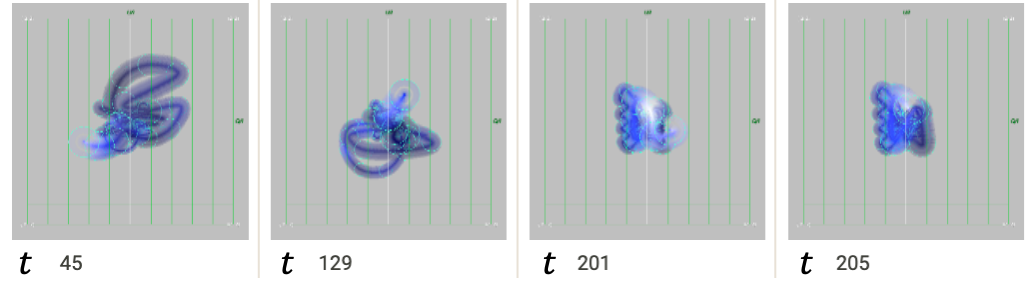
\includegraphics[width=.85\linewidth]{figures/flareDetectiondemodataResults.png}
    \caption{Flare detection results for our synthetic data. The results match the four red data samples in Fig.~\ref{fig:synthesisData}~(a).}
    \label{fig:flareDetection}
\end{figure}
\begin{figure}[tb]
    \centering
    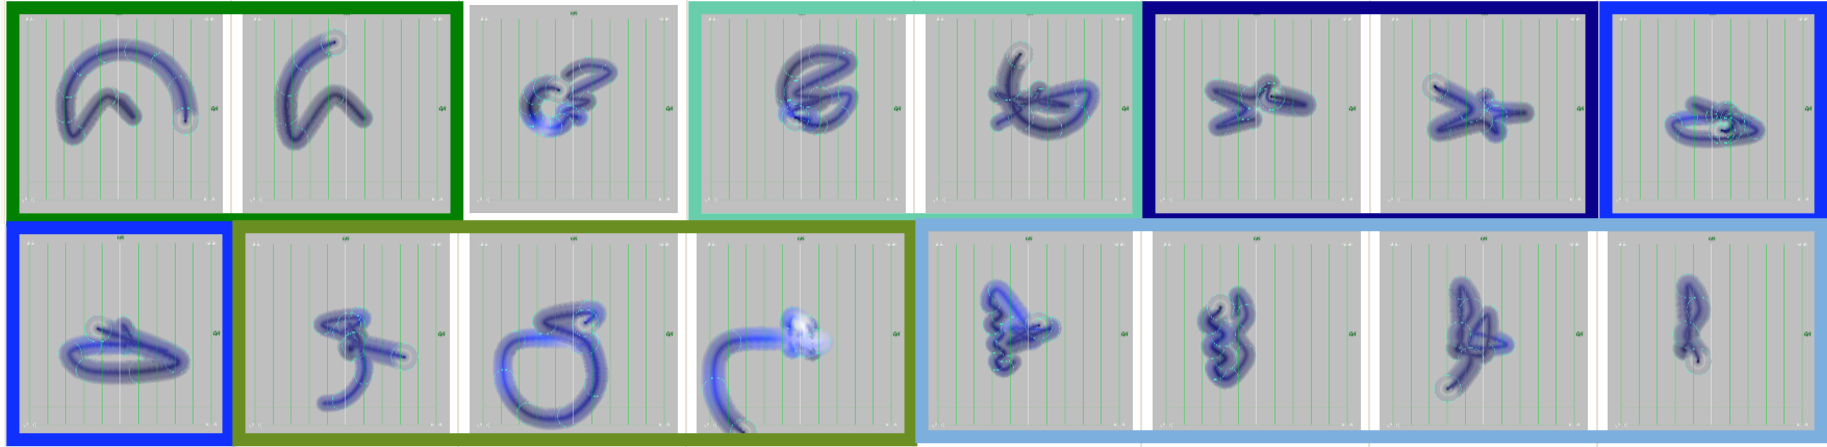
\includegraphics[width=\linewidth]{figures/rotationDetectiondemodataResultsOR.png}\\
    \footnotesize{\sf(a) Previous rotation detection method~\cite{Fujishiro2018}.}\\
    \vspace{5px}
    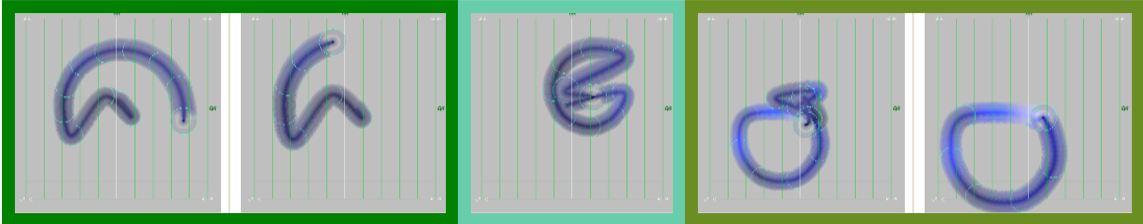
\includegraphics[width=.8\linewidth]{figures/rotationDetectiondemodataResults.png}\\
    \footnotesize{\sf(b) Our improved method.}
    \caption{Rotation detection results for our synthetic dataset in Fig.~\ref{fig:synthesisData}. 
        The outline color corresponds to the color in Fig.~\ref{fig:synthesisData}~(b).
        Our previous method detected narrow/rough-edged patterns and noise (blue), 
        whereas our improved method detected only large rotations (green).}
    \label{fig:rotationResults}
\end{figure}

\textsf{Experimental results.\ } We applied the flare detection method to our synthetic data.
We set $K$ and $h$ to 3 and 1, respectively.
Fig.~\ref{fig:flareDetection} presents the flare detection results.
The four data samples were detected as flares,
which completely coincide with the deliberately generated peaks that are highlighted in orange in Fig.~\ref{fig:synthesisData}~(a).

\subsection{Rotation Detection}\label{sec:rotationDetection}
Polarization rotation is another important observed behavior of blazars. 
Astronomers do not yet agree on whether rotation is an actual feature or just a result of random variations of polarization.
To validate their hypotheses, they scrutinize correlations between polarization and other properties at the time interval.
They typically have been analyzing the time variation of $PA$ to identify rotations~\cite{Ikejiri2011, Uemura2017},
but the rotation center will not be located at the origin of the Stokes plane ($(q, u) = (0, 0)$) when there are multiple polarized components in the sky.
Thus, estimating a rotation only through $PA$ may not allow astronomers to adequately understand its behavior.
Our rotation detection is capable of addressing any rotations regardless of the position of the rotation center.

We use a sliding window approach that allows users to manually define the length of the time interval for the sliding window. Based on feedback from astronomers~\cite{Sasada2012}, we set the default window size to be between three and four weeks.

The computation of the rotation angle is divided into the following seven steps:
\begin{enumerate}[nosep, label=\textsl{Step \arabic*}:, ref=\textsl{Step \arabic*}, align=parleft, leftmargin=*]
    \item \textsl{Compute the weighted means ($\overline{q}, \overline{u}$) of $q$ and $u$ at the time interval};\label{algo:rotationMean}
    \item \textsl{Compute the standard deviations ($\sigma_{q}, \sigma_{u}$) of $q$ and $u$ at the time interval}; \label{algo:rotationStd}
    \item \textsl{Convert the rectangular coordinates ($q-u$ domain) to polar coordinates ($r - \theta$ domain) with its origin shifted to $(\overline{q}, \overline{u})$}; \label{algo:rotationPolar}
    \item \textsl{Filter out time intervals whose $\sigma_{q}$ or $\sigma_{u}$ is smaller than the standard deviations of the entire dataset}; \label{algo:rotationFilter}
    \item \textsl{Compute the difference ($\theta_{\rm diff}$) of the $\theta$'s of two consecutive data samples}; \label{algo:rotationDiff}
    \item \textsl{Sum $\theta_{\rm diff}$'s to yield $\theta_{\rm sum}$}; \label{algo:rotationSum}
    \item \textsl{Check whether $\theta_{\rm sum}$ is larger than the user-specified threshold for the total rotation angle}. \label{algo:rotationThreshold}
\end{enumerate}
We regard $\overline{q}$ and $\overline{u}$ as a rotation center. 
To avoid misleading effects of outliers and unexpected values at the edges of a time interval,
smaller weights are assigned to both ends of the time interval according to a Gaussian distribution at \ref{algo:rotationMean}.
Note that users are allowed to adjust these weight ratios.
To avoid misclassifying time intervals with large $q$ or $u$ variance and unlike rotations as rotation candidates,
we have improved upon our previous rotation detection method~\cite{Sawada2018} on the basis of feedback from two astronomers at Hiroshima University~\cite{Huang2019}.
To detect only large rotations, 
our new method is able to filter out time intervals in which \textbf{either} $\sigma_{q}$ \textbf{or} $ \sigma_{u}$ is smaller than the standard deviation of the entire dataset. 
Note that this and other provided filtering constraints also allow for discovery of small or narrow rotations, such as the red and blue patterns in Fig.~\ref{fig:synthesisData}~(b).
At \ref{algo:rotationDiff}, we cannot compute $\theta_{\rm diff}$ simply by subtracting the $\theta$'s of consecutive observations 
due to the range constraint on $\theta_{\rm diff}$ (i.e., $\theta_{\rm diff} \in [0, 2\pi]$). 
For example, when two successive data samples are located in the first and fourth quadrant of the Stokes plane, 
we need to consider whether to take the clockwise or counterclockwise direction as $\theta_{\rm diff}$. 
We determine the rotation direction 
by checking increasing/decreasing tendency in $\theta$'s with exponential smoothing~\cite{Brown1956}.
It forecasts the next value according to past observations by assigning larger weights to more recent observations.
In this way, it addresses the uncertainty about the rotation direction and make results more feasible (\textbf{T1}).
We estimate the variation trend of $\theta$ and
then define the angle in the predicted rotation direction as $\theta_{\rm diff}$.
Users can set an arbitrary angle as a threshold parameter at \ref{algo:rotationThreshold}.

\textsf{Experimental results.\ } To compare our novel algorithm with the previous rotation detection algorithm~\cite{Sawada2018}, we applied both to our synthetic data.
As the results in Fig.~\ref{fig:rotationResults}~(a) show, 
the previous algorithm detected not only large rotations (green patterns in Fig.~\ref{fig:synthesisData}~(b)) but also narrow or rough-edged patterns (blue).
The improved algorithm more accurately detected only time intervals in which the polarization values dynamically rotate (green), as shown in Fig.~\ref{fig:rotationResults}~(b).